\section{Étude de performances}

\begin{frame}
	\frametitle{Les Parsers}
	\begin{center}
	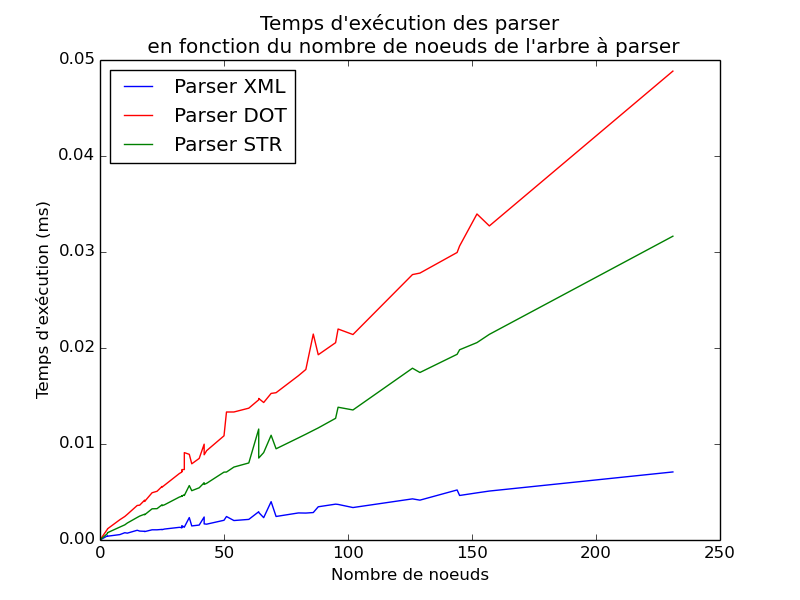
\includegraphics[height=7cm]{execTimeParsers}
	\end{center}
\end{frame}

\begin{frame}
	\frametitle{Calcul des coordonnées}
	\begin{center}
	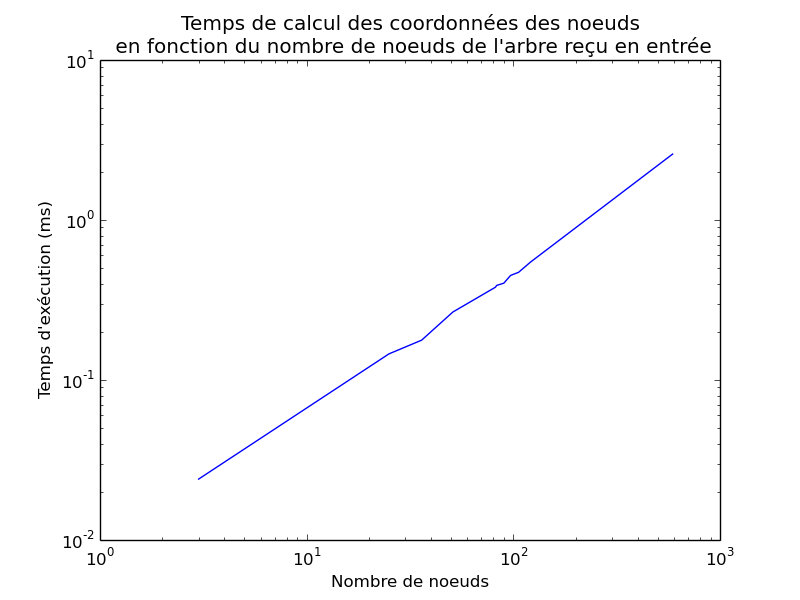
\includegraphics[height=7cm]{execTimeCoord}
	\end{center}
\end{frame}

\begin{frame}[allowframebreaks]
	\frametitle{Générateurs}
	\begin{center}
	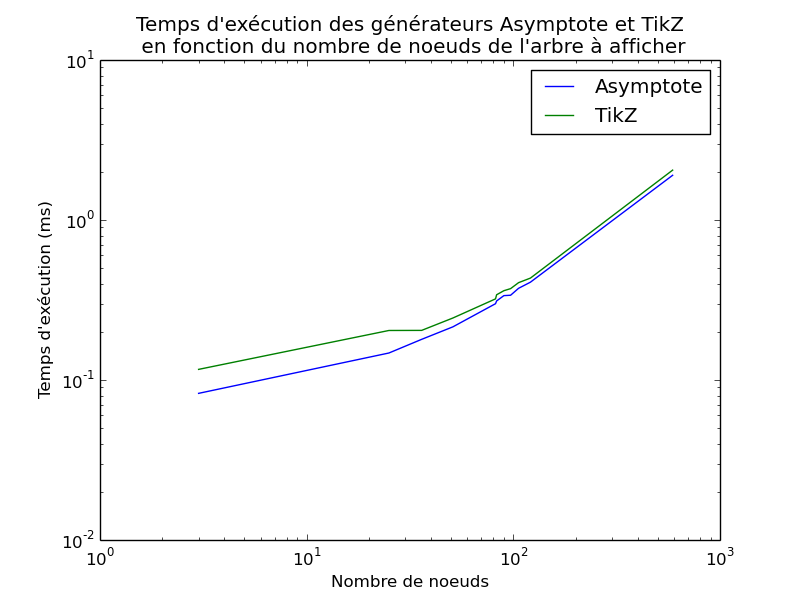
\includegraphics[height=7cm]{execTimeGenerators}
	\end{center}
	\begin{center}
	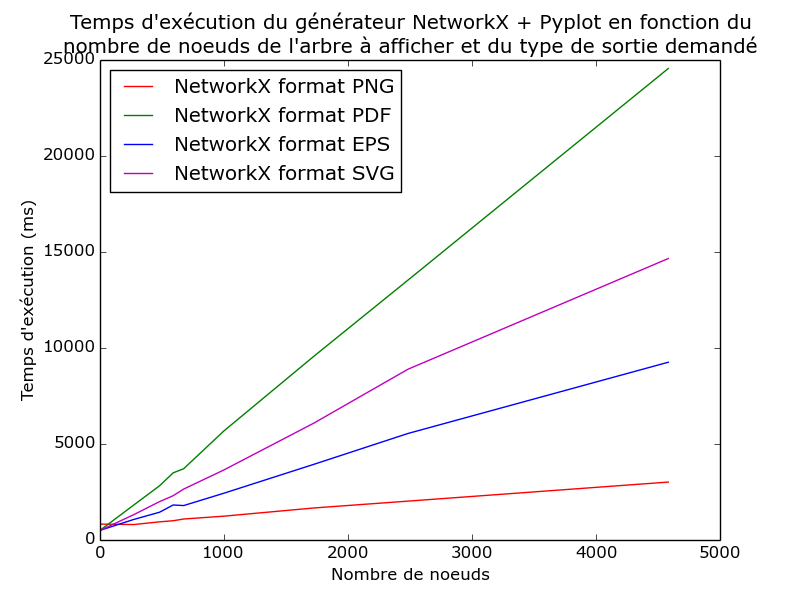
\includegraphics[height=7cm]{execTimeNX}
	\end{center}
\end{frame}

\begin{frame}
	\frametitle{GraphViz vs TreeDisplay}
	\begin{center}
	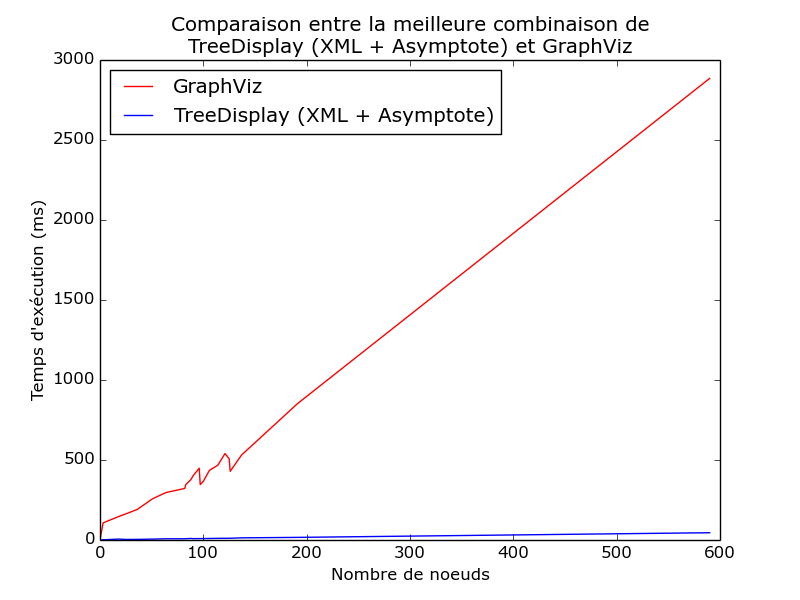
\includegraphics[height=7cm]{execTimeGV}
	\end{center}
\end{frame}



%\chapter{Étude de performances}
%
%\paragraph{} Avant toute chose, il est important de préciser que les tests effectués ci-dessous ont été réalisés sans aucun label. Comme expliqué précédemment, nous pouvons considérer que si la taille des labels est constante, la complexité des algorithme ne dépendra que du nombre de n\oe uds compris dans l'arbre. C'est donc l'hypothèse que nous faisons ici.
%
%	\section{Comparaison des temps d'exécution des différents parsers.}
%	
%\begin{center}
%
%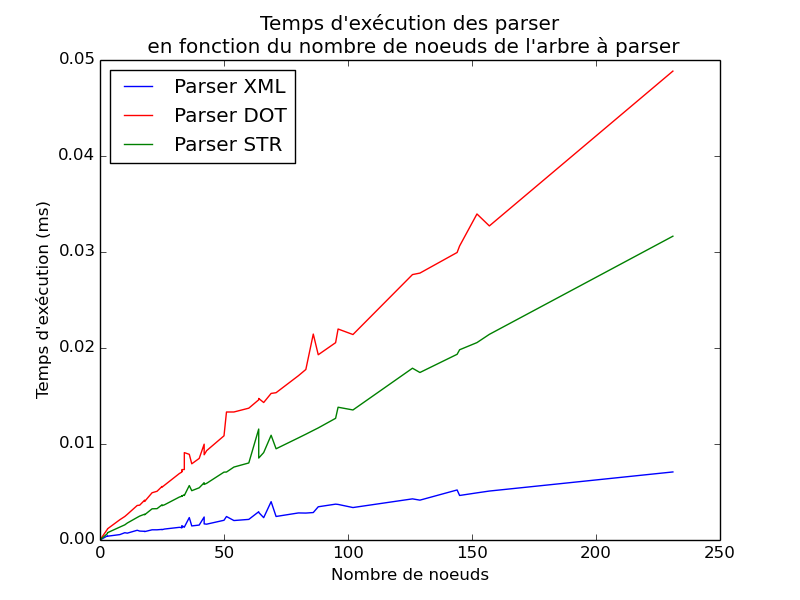
\includegraphics[width=\columnwidth]{execTimeParsers}
%
%\end{center}
%
%\paragraph{} Comme on avait pu le déduire précédemment, on peut observer que les parser ont une complexité linéaire. Ce qu'il ressort également de cette comparaison, c'est que le parser XML est le plus efficace des trois. Cela est certainement du au fait que nous utilisons un module interne à Python pour traiter le fichier d'entrée. En effet, les modules internes des langages sont généralement bien optimisés car pensés pour le langage concerné. De plus, en à peine une dizaine de secondes, nous pouvons parser un arbre contenant un million de n\oe uds.
%
%	\section{Évolution du temps de calcul des coordonées en fonction du nombre de n\oe uds de l'arbre.}
%	
%\begin{center}
%
%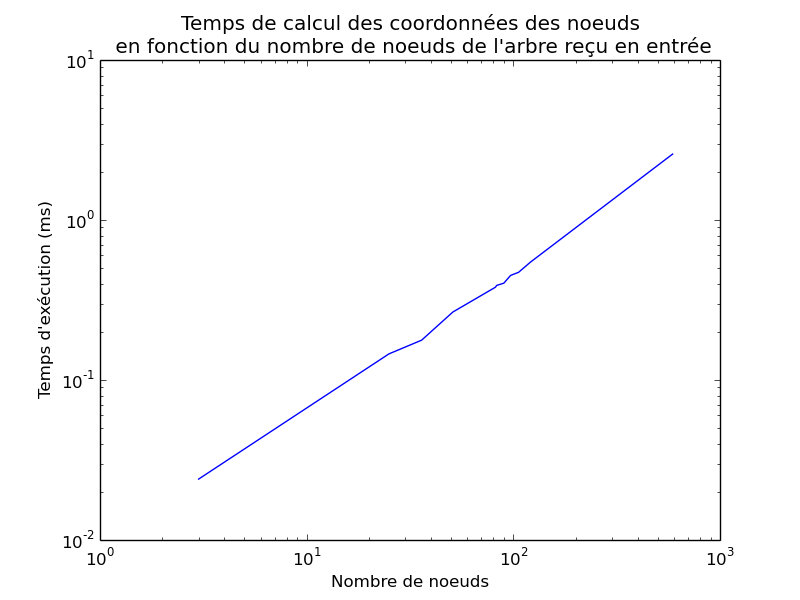
\includegraphics[width=\columnwidth]{execTimeCoord}
%
%\end{center}
%
%\paragraph{} Cette fois encore, le temps d'exécution de la méthode est d'une complexité linéaire. Nous pouvons également supposer, en observant l'évolution de la courbe, que pour un million de n\oe uds, nous n'aurions besoin que d'à peine une seconde pour effectuer le calcul de coordonnées, ce qui est un excellent résultat.
%
%	\section{Comparaison des temps d'exécution des différents générateurs.}
%
%\begin{center}
%
%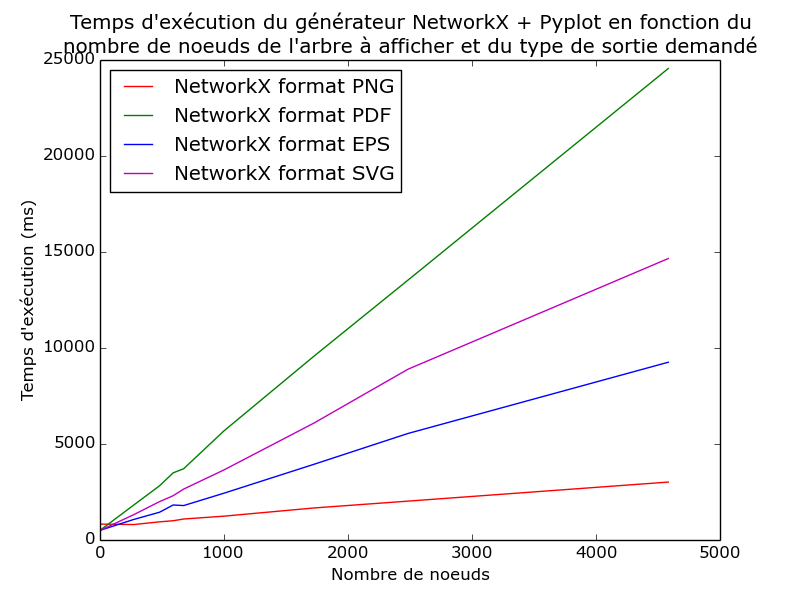
\includegraphics[width=\columnwidth]{execTimeNX}
%
%\end{center}
%
%\paragraph{} Nous comparons tout d'abord les différentes sorties gérées par NetworkX. Nous observons que nous sommes toujours en complexité linéaire, mais que le temps d'exécution est bien supérieur à ce qui peut être acceptable, avec plusieurs secondes pour seulement 5000 n\oe uds. Cependant, la complexité de ce générateur vient en grande partie du fait qu'il génère une image via MatplotLib. Ceci ralentit grandement l'exécution.
%	
%\begin{center}
%
%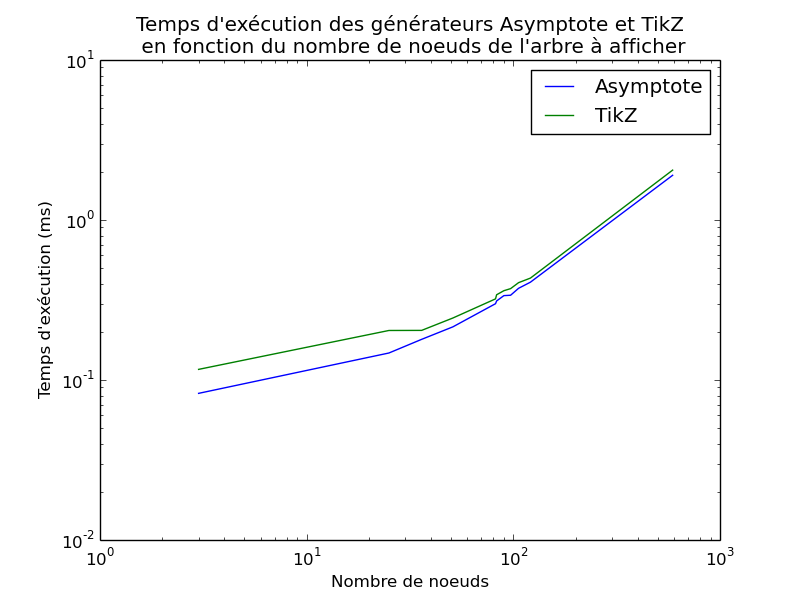
\includegraphics[width=\columnwidth]{execTimeGenerators}
%
%\end{center}
%
%\paragraph{} Contrairement à NetworkX, nous générons ici un fichier qui doit être recompilé. Ceci explique certainement en partie le fait que ce générateur soit plus efficace que le générateur NetworkX. Cependant, nous restons toujours en complexité linéaire.
%
%	\section{Comparaison des temps d'exécution entre GraphViz et la meilleur combinaison parser/générateur de TreeDisplay.}
%	
%\begin{center}
%
%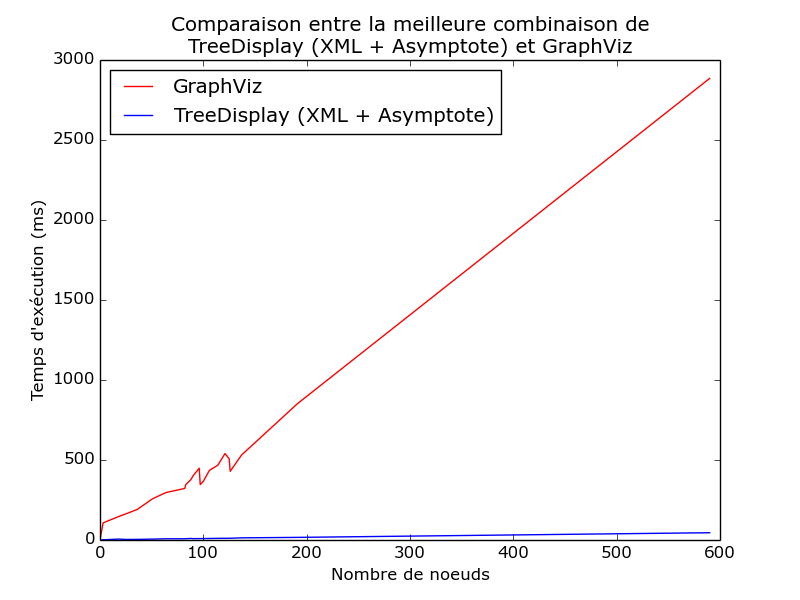
\includegraphics[width=\columnwidth]{execTimeGV}
%
%\end{center}
%
%\paragraph{} Nous comparons maintenant TreeDisplay dans sa meilleure combinaison possible de parser et de générateur de sortie, avec le visualiseur que nous avons cité en début de ce rapport : GraphViz. Il en ressort que TreeDisplay est bien plus puissant que GraphViz. Cependant, GraphViz gère des graphes de manière générale et fournit une image en sortie, et nous avons généré un fichier .tex à compiler. Ceci peut expliquer en partie la différence de performance.